% !TeX spellcheck = en_US

\chapter{Concept and Architecture}\label{chap:conarch}
\section{Concept}
In this section, the main concept of this work will be described.
The general structure of framework is represented in diagram \ref{fig:gen}.
% !TeX spellcheck = en_US

\begin{figure}
	\centering
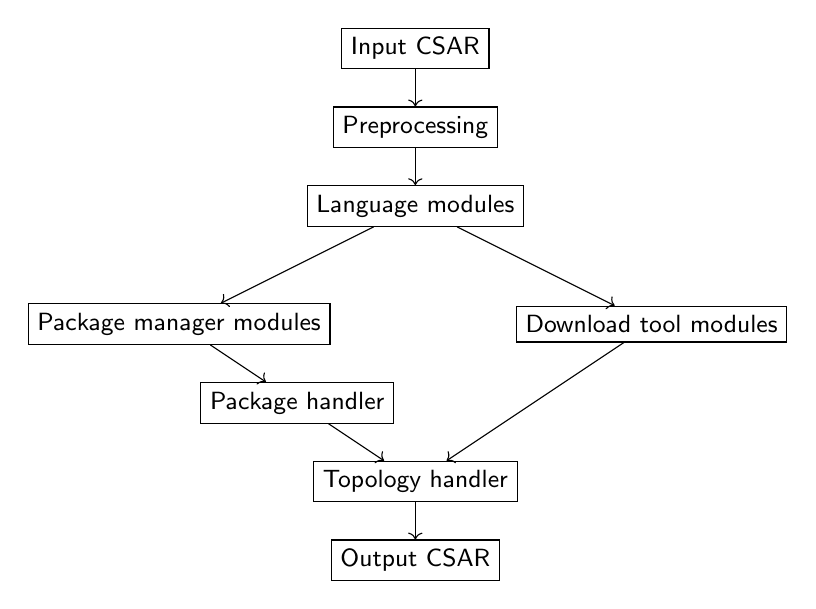
\begin{tikzpicture}
\node[draw] (in) at (0,1.5) {Input CSAR};
\node[draw] (pp) at (0,+0.5) {Preprocessing};
\node[draw] (lm) at (0,-0.5) {Language modules};
\node[draw] (pmm) at (-3,-2) {Package manager modules};
\node[draw] (dtm) at (+3,-2) {Download tool modules};
\node[draw] (ph) at (-1.5,-3) {Package handler};
\node[draw] (th) at (0,-4) {Topology handler};
\node[draw] (out) at (0,-5) {Output CSAR};
\draw [->] (in) -- (pp);
\draw [->] (pp) -- (lm);
\draw [->] (lm) -- (pmm);
\draw [->] (lm) -- (dtm);
\draw [->] (pmm) -- (ph);
\draw [->] (dtm) -- (th);
\draw [->] (ph) -- (th);
\draw [->] (th) -- (out);
\end{tikzpicture} 
\caption{The general description of the software's work flow} 	\label{fig:gen}
\end{figure}


\subsection{Analysis existing TOSCA-Topology}\label{subs:analyse}
To properly update the \gls{tosca} topology, it is necessary to add the references from nodes where external references were to newly created nodes, which resolve the external references. 
Artifacts belong to Node Types, but only Node Templates in the same Service Template can be referenced.  
It means that  Service Templates where the Node Templates with external references are instantiated must be found.
The Pointers to Artifacts are contained by Artifact Templates, which are used by Node Type Implementations.
By composing all the information a simple references chain can be built:\\
$Artifact$ $\rightarrow$ $Artifact$ $Template$ $\rightarrow$ $Node$ $Type$ $Implementation$ $\rightarrow$ $Node$ $Type$\\ $\rightarrow$ $Node$ $Template$ $\rightarrow$ $Service$ $Template$\\
Now consider the references in more detail. 
\begin{itemize}
	\item $Artifact$ $\rightarrow$ $Artifact$ $Template$\\
	An Artifact can be referenced by several Artifact Implementations. (Despite the fact that this is a bad practice.)
	\item  $Artifact$ $Implementation$ $\rightarrow$ $Node$ $Type$ $Implementation$ \\
	The same way an Artifact Template can be used by several Node Type Implementations.
	\item $Node$ $Type$ $Implementation$ $\rightarrow$ $Node$ $Type$ \\
	A Node Type Implementation can describe an implementation of only one Node Type.
	\item  $Node$ $Type$ $\rightarrow$ $Node$ $Template$\\
	Each Node Type can have any number of Node Templates.
	\item  $Node$ $Template$ $\rightarrow$ $Service$ $Template$\\
	But each Node Template is instantiated only once.
\end{itemize}
Thus structure can be described by a tree with an Artifact as the root, and Service Templates as leaves (The example is on figure \ref{fig:script_serv}) and will be called the internal dependencies tree.
% !TeX spellcheck = en_US
\usetikzlibrary{calc,arrows.meta,positioning}
\tikzset{
    every node/.style={font=\sffamily\small},
    main node/.style={shape=rectangle, rounded corners,
    	draw, align=center,
    	top color=white, bottom color=blue!20}
}

\begin{figure}
	\centering
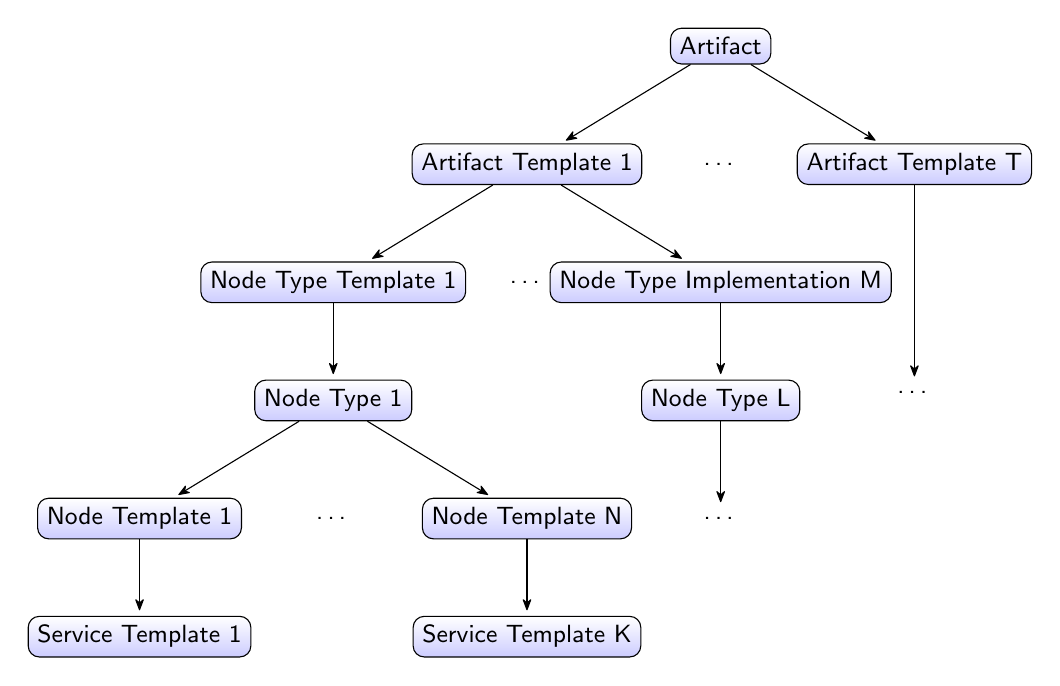
\begin{tikzpicture}[sibling distance=14em,->,>={Stealth[round,sep]},shorten >=1pt,auto,node distance=25mm]
    \node[main node] (1) {Artifact}
    child { node[main node](3) {Artifact Template 1} 
    	child { node[main node] (6) {Node Type Template 1} 
    			child { node[main node] (8) {Node Type 1} 
    				child { node[main node]  (11) {Node Template 1} 
    					child { node[main node] (13) {Service Template 1}}  
    				}
    				child { node[main node]  (12) {Node Template N} 
    					child { node[main node] (14) {Service Template K}}
    				}
    			}
    	}
    	child { node[main node] (7) {Node Type Implementation M} 
    		child { node[main node] (9) {Node Type L} 
    			child { node  (10) {\ldots} }
    		}
    	}
    }
    child { node[main node] (4) {Artifact Template T}  
    child { node (5) [below =of 4]{\ldots}}
	};

    \node at ($(3)!.5!(4)$) {\ldots};
    \node at ($(6)!.5!(7)$) {\ldots};
    \node at ($(11)!.5!(12)$) {\ldots};
    
\end{tikzpicture} 
\caption{An example tree describing how to find Service Templates and Node Templates for the given script} 	\label{fig:script_serv}
\end{figure}
%Of course it is possible to move in opposite direction, starting from a Node and moving toward scripts, but this method brings additional complexity. 
An additional problem is in the reference between a Node Type and a Node Type Implementation.
Node Type can have several Node Type Implementations, but which one will be used will be determined only during the deployment. 
The chosen solution to this problem is to use each Node Type Implementation in hope, that they will not conflict.\\
%The method presented above can uniquely determine Node Templates and Service Template for a given script.
%Of course it is not guaranteed that found Node Type Implementation will be used during deployment, but we can't do anything with this. 
The following steps can be executed during the preprocessing, to identify the necessary dependencies.
\begin{itemize}
	\item Find all Artifact Templates to build references from Artifacts to Artifact Templates.
	\item Find all Node Type Implementations. Because they contain both the Node Type and Artifact Templates, then the dependency from Artifact to Node Types can be built.
	\item Find all Service Templates and in them contained Node Templates. Any Node Template contains a reference to Node Type, what is useful for building a dependency from Artifact to Node Template.
\end{itemize} 
In this way, the required internal dependencies tree can be built (script $\rightarrow$ Node Template and script $\rightarrow$ Service Template).
\subsection{Find external dependencies}
Analysis for external references.
Unfortunately, it is impossible to identify all possible external dependencies, even when one language and one package manager are used (example in algorithm \ref{alg:unreadable}).
\begin{Algorithmus} 
	\caption{Unreadable bash script}
	\label{alg:unreadable}
	\begin{algorithmic}
		\State	\#!/bin/bash
		\State	$\textbf{set } line = $abcdefgijklmnoprst
		\State	$\textbf{set } word1 = \$\{line:0:1\}\$\{line:14:1\}\$\{line:17:1\}$ 
		\State  $\textbf{set } word2 = \$\{line:6:1\}\$\{line:4:1\}\$\{line:17:1\}$
		\State  $\$word1\$-\$word2\$$ install package
	\end{algorithmic}
\end{Algorithmus}   
Since this work is aimed at creating of the easily expanded and supplemented tool, initially only basic usage of package managers will be considered.
% and complimented only when it will be necessary. 
Ease of adding modules to the framework will proof the correctness of architecture.
At the beginning, the most popular combination will be implemented: the $bash$ script with the $apt-get$ package manager.
This simple and powerful tool allows to install, delete or update the set of packages in one line.
After the modules for this combination will be implemented, new languages and package managers should be added.
\subsection{Representing downloaded packages in TOSCA-Topology} \label{subs:repres}
A package node denotes to the defined and instantiated element of \gls{tosca} topology, the purpose of which is to install the package.
The adding of new package nodes to TOSCA topology can be divided into several steps.
\begin{itemize}
	\item Add definitions for common elements, like Artifact Types or Relationship Types. 
		This can be done once at the preprocessing stage.
	\item The package node main definition will be represented by a Node Type. 
		%There will be described that this node must be installed.
	\item Artifacts (The downloaded data and the installation script) will be referenced by Artifact Templates.
	\item Node Type Implementation will combine the artifacts.
	\item Node Template will instantiate a package in the corresponding Service Templates.
		To determine corresponding Service Template the preprocessing described in the section \nameref{subs:analyse} will be used.
	\item Reference Template will provide topology information, allowing the observer (a user or a runtime environment) to determine, for which nodes the package must be installed.
		References will be created from nodes needing the package to Node Templates of created package nodes.
\end{itemize}
\subsection{Determining architecture of a final platform}
An another problem appears during choosing the architecture of the device where packages will be installed.
Unfortunately, it is impossible to analyze the structure of any CSAR and give an unambiguous answer to the question, on which architecture which node will be deployed.
There are many pitfalls here.\\
A single Service Template can use several physical devices with different architectures.
One Implementation Artifacts can be referred by different Node Types and Node Templates and instantiated on different platforms.
This way one simple Implementation Artifact with a bash script containing "$apt$-$get$ $install$ $python$" command can be deployed on different devices within one Service Template (for example with the arm, amd64 and i386 architectures) and will result in the loading and installation of three different packages. 
For an end user, the ability to use such a simple command is a huge advantage, but for the framework, it can greatly complicate analysis.
The following methods of architecture selection were designed.
\begin{itemize}
	\item $Deployment$ $environment$ analysis\\
	The script can analyze the system where it was started (for example using the "$uname$~$-a$" command) and depending on the result, it will install the package corresponding to the system's architecture.
	\item $Unified$ $architecture$\\
	The architecture will be defined by the user for a whole CSAR.
	\item $Artifact$ $specific$ $architecture$\\
	The architecture will be defined separately for each artifact.
\end{itemize}
\subsubsection*{Analysis of methods}
Unfortunately, the $deployment$ $environment$ $analysis$, which at first sight seems to be the most reliable solution, brings many additional problems.
Packages for different platforms can differ not only by architecture but also by the version and the list of dependencies.
As a consequence, a chaos can be produced by mirroring these different packages with different versions to the \gls{tosca}-topology.
The only robust solution seems to be to create for each installed package a set of archives (one archive for each architecture), containing the entire dependency tree for the given package.
But this approach contradicts one of the main ideas of this work: the dependencies trees should be mapped to the topology.\\
The $artifact$ $specific$ $architecture$ method carries an additional complexity to the user of the framework.
It will obligate a user to analyze each artifact and decide on which architecture it will be executed. 
This can be complicated by the fact that the same artifact can be executed on different architectures.\\
The method of the $unified$ $architecture$ was chosen, as the simplest and easiest to implement.
If it will be necessary, this method can be easily expanded to the $artifact$ $specific$ $architectures$ method (By removing the user input at start, and choosing an architecture for each artifact separately.) or to $deployment$ $environment$ $analysis$ (By downloading packages for all available architectures and adding the architecture determining algorithm to the installation scripts.).

\subsection{Extensibility}
The framework should handle different languages, each of them can support various package managers.
This principle can be illustrated by a figure \ref{fig:lang_pm}.
% !TeX spellcheck = en_US

% We need layers to draw the block diagram
\usetikzlibrary{calc,positioning}

% Define a few styles and constants
\tikzstyle{entry}=[draw, fill=green!20, minimum height=2.0em, text width=8.0em]
\tikzstyle{ann} = [above, text width=5em]
\tikzstyle{framework} = [entry, text width=35em, fill=red!20, 
minimum height=19em, rounded corners]
\tikzstyle{lang} = [entry, text width=9em, fill=blue!20, 
minimum height=16em, rounded corners]
\def\blockdist{2.3}
\def\edgedist{2.5}

\begin{figure}
	\centering
\begin{tikzpicture}
\node (rr) [framework] {};
\node [xshift=+5mm, yshift=-2mm, below right] at (rr.north west) {\large References resolver framework };


\node (lang1) at ([xshift=-52mm,yshift=-4mm]rr) [lang] {};
\node [xshift=+3mm, yshift=-2mm, below right] at (lang1.north west) [text width=6em] {\large Language module 1 };
\node (lang2) at ([xshift=-7mm,yshift=-4mm]rr) [lang] {};
\node [xshift=+3mm, yshift=-2mm, below right] at (lang2.north west) [text width=6em] {\large Language module 2 };
\node (langn) at ([xshift=+52mm,yshift=-4mm]rr) [lang] {};
\node [xshift=+3mm, yshift=-2mm, below right] at (langn.north west) [text width=6em] {\large Language module N };  
\node at ($(lang2)!.5!(langn)$) {\ldots};

\node (l1pm1) at ([yshift=+15mm]lang1) [entry] {Package manager module};
\node (l1pm2) at ([yshift=0mm]lang1) [entry] {Package manager module};
\node (l1pmn) at ([yshift=-25mm]lang1) [entry] {Package manager module};
\node at ($(l1pm2)!.5!(l1pmn)$) {\vdots};

\node (l2pm1) at ([yshift=+15mm]lang2) [entry] {Package manager module};
\node (l2pm2) at ([yshift=0mm]lang2) [entry] {Download tool module};
\node (l2pm3) at ([yshift=-13mm]lang2) [entry] {Package manager module};
\node (l2pmn) at ([yshift=-25mm]lang2) [entry] {Package manager module};
%\node at ($(l2pm2)!.5!(l2pmn)$) {\vdots};

\node (lnpm1) at ([yshift=+15mm]langn) [entry] {Package manager module};
\node (lnpm2) at ([yshift=0mm]langn) [entry] {Package manager module};
\node (lnpm3) at ([yshift=-13mm]langn) [entry] {Download tool module};
\node (lnpmn) at ([yshift=-25mm]langn) [entry] {Download tool module};
%\node at ($(lnpm2)!.5!(lnpmn)$) {\vdots};


\end{tikzpicture} 
\caption{An example scheme representing several language modules containing package manager modules} 	\label{fig:lang_pm}
\end{figure}

\subsection{Result's checking}
Checking the output of the framework is an important stage in the development of the program.
It is necessary to verify both the overall validity of the output \gls{csar} and the possibility to deploy the output \gls{csar}.
To test for overall correctness it is possible to use $winery$ tool from OpenTOSCA.
This tool for creating and editing archives is also great for visualizing results.
Checking the deployment of the CSAR can be dome manual by starting corresponding commands.

\section{Architecture}\label{sec:arch}
This section will present the architecture of the framework and a description of its elements.
The main elements are $references$ $resolver$, $language$ $modules$, $package$ $manager$ $modules$, $package$ $handler$ and $topology$ $handler$.

\subsection{CSAR handler} \label{subs:casr_h}
\gls{ch} provides access to \gls{csar} and maintains CSAR consistency. 
It describes the process of adding new files (to handle the metadata), decompression, architecture processing, etcetera.

\subsection{References resolver} \label{subs:RR}
This is the main element, the execution of which can be divided into three stages: $preprocessing$, $processing$, $finish$. \\
At the begin the $preprocessing$ will be executed for decompression, adding files (The list with common files, which are added during preprocessing is described in the section \ref{subs:repres}) and generating internal dependencies trees (the generation is described in the section \ref{subs:analyse}).
Figure \ref{fig:preproc} illustrates the stages of the preprocessing.
% !TeX spellcheck = en_US

\usetikzlibrary{calc,arrows.meta,positioning,arrows}
\tikzset{
    every node/.style={font=\sffamily\small},
    main node/.style={shape=rectangle, rounded corners,
    	draw, align=center,
    	top color=white, bottom color=blue!20}
}

\tikzstyle{entry}=[draw, fill=green!20, minimum height=2.2em, text width=7em]
\tikzstyle{myentry}=[draw, fill=Dandelion!20, minimum height=2.5em, text width=7em]
\tikzstyle{ann} = [above, text width=5em]
\tikzstyle{frame} = [entry, text width=10em, fill=red!20, 
minimum height=17em, rounded corners]
\tikzstyle{csar_content} = [entry, text width=9em, fill=blue!20, 
minimum height=14em, rounded corners]
\tikzstyle{out_content} = [entry, text width=10em, fill=blue!20, 
minimum height=17em, rounded corners]
\def\blockdist{2.3}
\def\edgedist{2.5}
\begin{figure}
	\centering
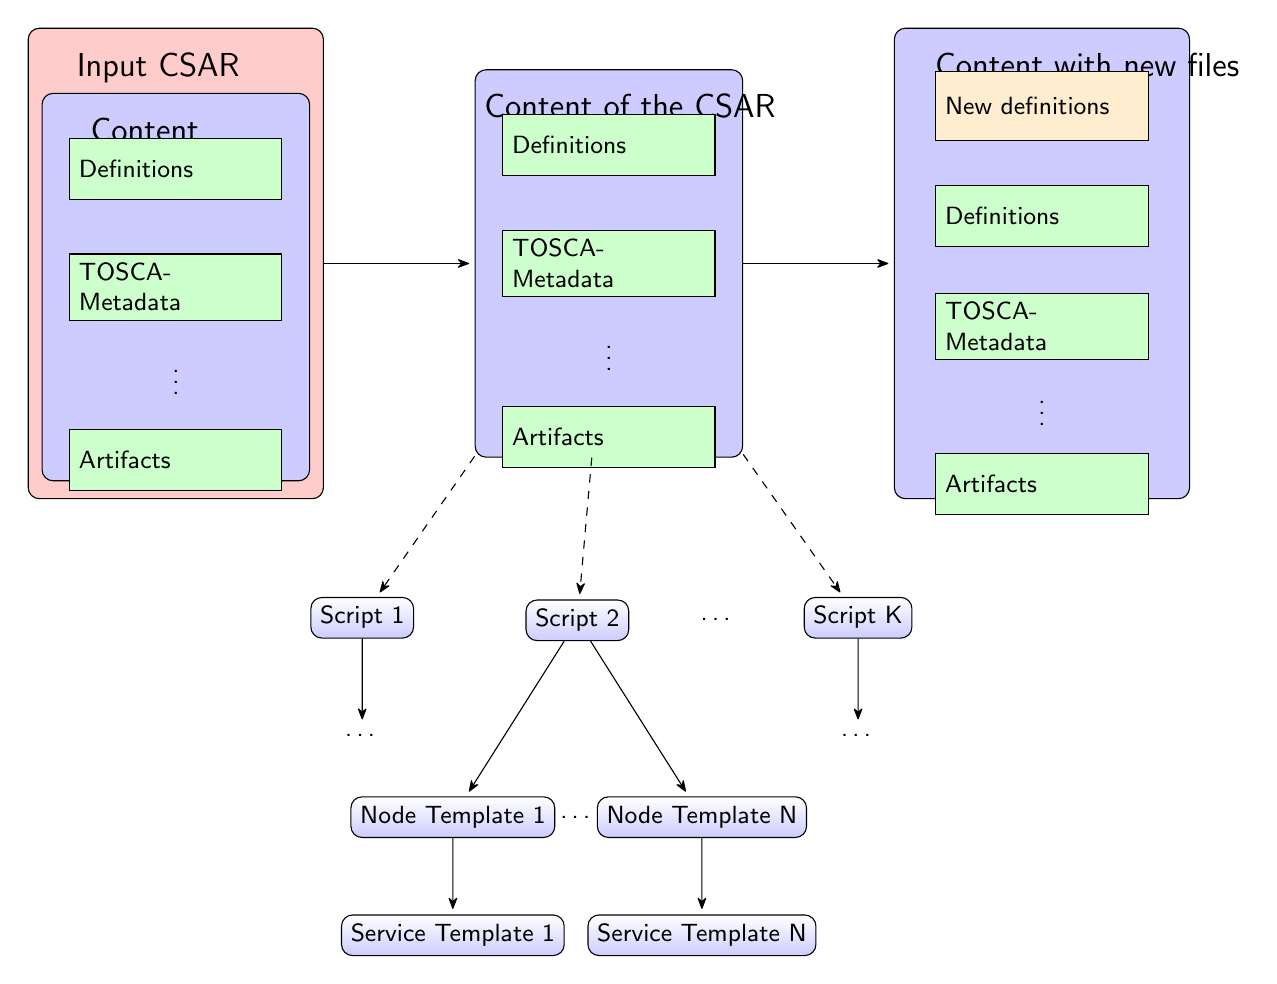
\begin{tikzpicture}[sibling distance=9em,->,>={Stealth[round,sep]},shorten >=1pt,auto,node distance=25mm]


\node (csar_frame) [frame] {};
\node [xshift=+5mm, yshift=-2mm, below right] at (csar_frame.north west) {\large Input CSAR};

\node (csar_content) at ( [yshift=-3mm]csar_frame) [csar_content] {};
\node [xshift=+5mm, yshift=-2mm, below right] at (csar_content.north west) {\large Content};

\node (l2pm1) at ([yshift=+15mm]csar_content) [entry] {Definitions\\};
\node (l2pm2) at ([yshift=0mm]csar_content) [entry] {TOSCA-Metadata\\};
\node (l2pmn) at ([yshift=-22mm]csar_content) [entry] {Artifacts\\};
\node at ($(l2pm2)!.5!(l2pmn)$) {\vdots};
    
\node [right of=csar_frame, xshift=30mm](dc_frame) [csar_content] {};
\node [xshift=+0mm, yshift=-2mm, below right] at (dc_frame.north west) {\large Content of the CSAR };
\draw [->] (csar_frame) -- (dc_frame);
\node (2pm1) at ([yshift=+15mm]dc_frame) [entry] {Definitions\\};
\node (2pm2) at ([yshift=0mm]dc_frame) [entry] {TOSCA-Metadata\\};
\node (2pmn) at ([yshift=-22mm]dc_frame) [entry] {Artifacts\\};
\node at ($(2pm2)!.5!(2pmn)$) {\vdots};

\node [right of=dc_frame, xshift=30mm](my_frame) [out_content] {};
\node [xshift=+4mm, yshift=-2mm, below right] at (my_frame.north west) {\large Content with new files};
\draw [->] (dc_frame) -- (my_frame);
\node (3pmd) at ([yshift=+20mm]my_frame) [myentry] {New definitions\\};
\node (3pm1) at ([yshift=+6mm]my_frame) [entry] {Definitions\\};
\node (3pm2) at ([yshift=-8mm]my_frame) [entry] {TOSCA-Metadata\\};
\node (3pmn) at ([yshift=-28mm]my_frame) [entry] {Artifacts\\};
\node at ($(3pm2)!.5!(3pmn)$) {\vdots};


\node[below=of dc_frame,main node, node distance=10mm, xshift=-4mm, yshift=+7mm] (11) {Script 2}
child { node[main node, yshift=-10mm]  (n21) {Node Template 1} 
		child { node[main node] (s31) {Service Template 1}}  
}
child { node[main node, yshift=-10mm]  (n22) {Node Template N} 
	child { node[main node] (s32) {Service Template N}}  
};
\draw [dashed,->] (dc_frame) -- (11);
\node[below left=of dc_frame,main node,xshift=+10mm] (12) {Script 1}
child { node  {\ldots} 
};
\draw [dashed,->] (dc_frame) -- (12);
\node[below right=of dc_frame,main node, xshift=-10mm] (13) {Script K}
child { node  {\ldots} 
};
\draw [dashed,->] (dc_frame) -- (13);
\node at ($(11)!.5!(13)$) {\ldots};
\node at ($(n21)!.5!(n22)$) {\ldots};

\end{tikzpicture} 
\caption{Preprocessing: decompression, addition of common definitions and generation of internal dependencies trees} 	\label{fig:preproc}
\end{figure}
During the $processing$, all $language$ $modules$ will be activated, which are described in the next section. \\
To finish the work  all results will be packed back to the archive during the $finish$ stage.
\subsection{Language modules} \label{subs:archlm}
Each $language$ $module$ describes one language and helps to choose files written in the language.
As already mentioned above, during $processing$ stage $language$ $module$ analyzes all files one by one and checks its belonging to the specified language. 
Any files not belonging to the described language are filtered out.
The remaining files are transferred to this $language$ $module$'s $package$ $manager$ $modules$.
For example, a $Bash$ module can pass through only files with $".sh"$ extension and starting with the $"\#!/bin/bash"$ line.
\subsection{Package manager modules} \label{subs:archpmm}
$Package$ $managers$ $module$ finds external references, resolve them and transmit the package name to the package handler module, described in the next section.
Figure \ref{fig:lang_ph} illustrates data flow between languages, package managers, and package handler.
% !TeX spellcheck = en_US
\usetikzlibrary{calc,arrows.meta,positioning}
\tikzset{
    every node/.style={font=\sffamily\small},
    main node/.style={shape=rectangle, rounded corners,
    	draw, align=center,
    	top color=white, bottom color=blue!20},
    data node/.style={shape=rectangle,
    draw, align=center,
    top color=white, bottom color=red!20}
}

\begin{figure}
	\centering
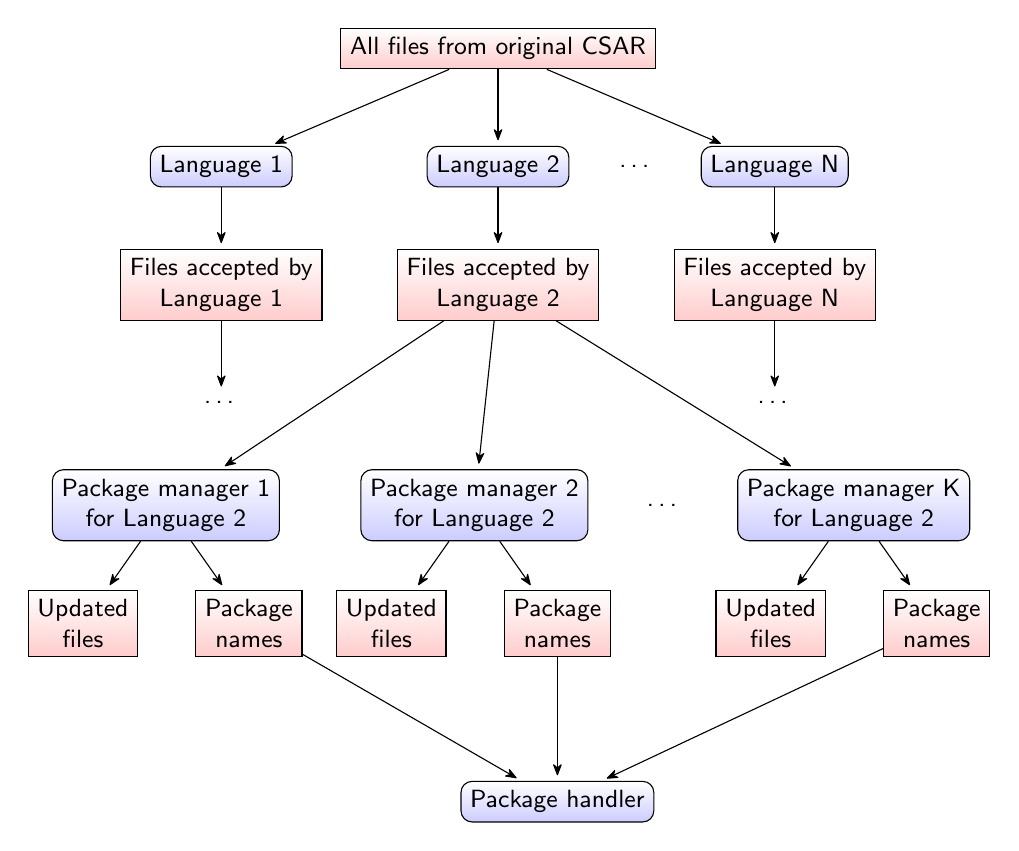
\begin{tikzpicture}[->,>={Stealth[round,sep]},shorten >=1pt,auto,level 1/.style={sibling distance=10em,node distance=25mm},
level 2/.style={sibling distance=8em,node distance=30mm},
level 3/.style={sibling distance=12em,node distance=30mm},
level 4/.style={sibling distance=6em,node distance=25mm},
level 5/.style={sibling distance=8em,node distance=25mm},
level 6/.style={sibling distance=8em,node distance=25mm}]
    \node[data node] (1)  {All files from original CSAR}
    child { node[main node](2) {Language 1} 
    	child { node[data node](21) {Files accepted by\\ Language 1} 
    		child { node {\ldots}}}}
	child { node[main node] (3) {Language 2}
		child { node[data node](31) {Files accepted by\\ Language 2} 
			child { node[main node, yshift=-13mm](32) {Package manager 1\\for Language 2} 
				child { node[data node](36) {Updated\\ files}}
				child { node[data node](37) {Package\\ names}}}
			child { node[main node, yshift=-13mm, xshift=-3mm](33) {Package manager 2\\for Language 2}
				child { node[data node](34) {Updated\\ files}}
				child { node[data node](35) {Package\\ names}}}
			child { node[main node, yshift=-13mm, xshift=+3mm](34) {Package manager K\\for Language 2}
				child { node[data node](38) {Updated\\ files}}
				child { node[data node](39) {Package\\ names}}}
			}
		}
    child { node[main node] (4) {Language N}
    	child { node[data node](41) {Files accepted by\\ Language N} 
    		child { node {\ldots}}}}
	;

	\node [main node,below, yshift=-20mm] at (35) (ph) {Package handler};
    \node at ($(3)!.5!(4)$) {\ldots};
    \node at ($(33)!.5!(34)$) {\ldots};
    \draw [->] (35) --(ph);
    \draw [->] (37) --(ph);
    \draw [->] (39) --(ph);
    
\end{tikzpicture} 
\caption{The data flow scheme between language modules, package manager modules and the package handler.} 	\label{fig:lang_ph}
\end{figure}

\subsection{Package Handler} \label{subs:archph}
$Package$ $handler$ becomes a package name, downloads a data for the package installation, transfer the package name to the $topology$ $handler$ and recursively repeats the actions for all depended packages.

\subsection{Topology Handler} \label{subs:archtop}
$Topology$ $handler$ adds a package to the topology. 
This includes adding new files and updating existing files. 
Necessary steps were described in section \ref{subs:repres}.